% !TeX program = xelatex
% !BIB program = bibtex
\documentclass[UTF8,a4paper,zihao=-4]{ctexart}

\usepackage{amsmath,amssymb,bm}
\usepackage{booktabs}
\usepackage{geometry}
\usepackage{graphicx}
\usepackage{hyperref}
\usepackage{caption}
\usepackage{subcaption}
\usepackage{float}
\usepackage{cite}
\usepackage{array}
\usepackage{tabularx}

\geometry{left=2.6cm,right=2.6cm,top=2.6cm,bottom=2.6cm}
\graphicspath{{figures/}{paper/figures/}}
\hypersetup{colorlinks=true,linkcolor=black,citecolor=black,urlcolor=black}
\captionsetup{font=small,labelfont=bf}
\setlength{\parskip}{0.35em}
\setlength{\emergencystretch}{2em}
\renewcommand{\arraystretch}{1.18}
\renewenvironment{abstract}
  {\par\small\noindent{\heiti 摘要：}}
  {\par\vspace{0.8em}\normalsize}

\title{\heiti 基于 VGGT-3DGS-BEV 的纯视觉教室精细照明调控方法研究}
\author{作者：待补充\\专业：待补充\\课程：待补充}
\date{}

\begin{document}
\maketitle

\begin{abstract}
在绿色低碳校园建设背景下，教学楼照明系统既影响公共建筑能耗，也影响课堂学习、板书观看和投影使用等教学体验。传统教室照明控制通常以房间级开关、定时控制、固定分区或人体红外感应为主，难以表达课桌面、黑板面、投影幕面、讲台和过道等不同教学工作表面的差异化需求。本文提出一种基于 VGGT 点图、3DGS 静态辅助和三维工作表面单元的纯视觉教室精细照明调控方法。方法首先将多相机图像中的语义掩码提升到三维空间，构建统一的工作表面 cell；随后利用 3DGS 提供静态背景、动态残差、可见性和基础反射外观辅助；在线阶段通过 Swin-Tiny-FPN 多任务感知估计人员占用、教学活动和当前光照；最后结合灯具贡献矩阵、环境光分离和目标需求函数，通过约束优化求解灯具亮度。为验证方法链路的可执行性，本文构建合成输入驱动的原型仿真程序，对 cell 索引、贡献矩阵、目标需求、控制向量和质量指标进行分析。结果表明，该方法能够在统一三维工作表面索引下形成从视觉感知到灯光控制的闭环，并为教室精细化节能照明提供一种可解释的研究路线。

\par\noindent{\heiti 关键词：}智能照明；纯视觉感知；VGGT；3D Gaussian Splatting；工作表面 cell；约束优化
\end{abstract}

\section{引言}

在绿色低碳校园建设背景下，教学楼照明系统既关系到公共建筑能耗，也直接影响课堂学习、板书观看和投影使用等教学体验。传统教室照明控制通常以房间级开关、定时控制、区域开关或人体红外感应为主，控制对象多为整间教室或固定灯区，难以区分学生课桌面、黑板面、投影幕面、讲台区域和过道等不同教学工作表面的实际需求。当教室内只有局部区域有人、窗边自然光已经充足、或课堂处于投影模式时，粗粒度控制容易造成无人区域过度照明；当学生书写、教师板书或局部讨论发生时，固定控制又可能无法保证关键任务表面的照明需求。

国内外关于智能照明控制的研究主要围绕建筑节能、视觉舒适、人员占用感知和日光利用展开。早期与工程应用较成熟的方案多采用人体存在传感器、照度传感器、定时开关和固定分区策略，通过判断空间是否有人、自然光是否充足以及是否处于使用时段来控制灯具开关或连续调光\cite{haq2014review,pandharipande2015smart}。这类方法结构简单、成本较低，适合教学楼、办公楼等大面积场景的基础节能控制。基于日光传感器的 daylight harvesting 方法可以在窗边自然光充足时降低人工照明输出，从而减少人工照明能耗\cite{delvaeye2016analysis}。部分研究进一步将传感器布设在灯具附近，形成 luminaire-based sensing 系统，使每个灯具能够根据局部占用和局部照度进行调节，提升分区控制的灵活性。

随着控制理论和智能优化方法的发展，国外研究开始从简单规则控制转向个性化照明、闭环调光和多目标优化控制。例如，有研究利用桌面照度传感器、窗帘控制和智能控制器，在满足用户个性化照明需求的同时利用自然光降低能耗；也有研究在学校建筑中比较不同 daylight dimming 控制系统的节能效果，说明教室照明控制不仅与灯具开关有关，还与窗边自然光、教室朝向、控制策略和使用时段密切相关。近年来，部分研究开始关注课堂场景中的视觉舒适和教学活动差异，例如利用高动态范围图像或监控摄像头估计教室亮度分布，并结合日光和人工照明控制改善课堂视觉环境\cite{budhiyanto2024visual}；也有研究从座位区域、投影使用和学生主观感受等角度评价大学教室视觉舒适\cite{chiou2020visual}，说明课堂照明不仅是能耗问题，也与学习活动和视觉任务密切相关。

国内关于教学楼和教室智能照明的研究与工程实践多集中在物联网传感器、单片机控制、ZigBee 或无线通信、人体红外检测、光敏电阻、照度采集和分区控制等方向。典型方案通常在教室内布设人体红外传感器和光照传感器，根据是否有人、环境光强和预设区域规则控制灯具开关或亮度；也有方案通过灯具分组、座位压力检测或人数统计实现按区域开灯，避免无人区域长时间照明。这些方法能够降低传统“整间教室统一开灯”造成的能源浪费，也具有较好的工程可实施性。

总体来看，现有智能照明控制研究已经在占用感知、日光利用、分区调光和节能优化方面形成了较成熟的技术路线，但仍存在三个不足：第一，控制粒度多停留在房间级、灯组级或固定分区级，难以精确表达课桌面、黑板面、投影幕面等不同教学任务表面的照明需求；第二，人员感知多关注“是否有人”或“有多少人”，对听课、书写、板书、投影观看等课堂活动差异考虑不足；第三，现有系统通常将感知结果直接转化为开关灯或调光规则，缺少从人员活动、当前光照、环境光贡献到灯具控制量之间的统一建模。因此，面向绿色低碳校园的教室照明控制仍需要进一步从粗粒度分区控制走向面向教学任务和真实工作表面的精细化调控。

本文的目标是在输入仅有多相机图像的条件下，探索一种具有创新性、解释性和闭环控制能力的纯视觉教室精细照明调控方法。本文首先利用 VGGT 点图\cite{wang2025vggt}和语义掩码构建三维工作表面；随后借鉴神经场景表示的发展脉络\cite{mildenhall2020nerf}，使用 3DGS\cite{kerbl2023gaussian}作为静态外观和可见性辅助模块；在线阶段采用 Swin-Tiny-FPN\cite{liu2021swin,lin2017fpn}共享视觉 backbone 和占用、活动、光照三个任务 head 输出 $O_t(i)$、$A_t(i,k)$ 和 $L_t(i)$；最后结合灯具贡献矩阵 $M(i,g)$、环境光估计 $L_{day,t}(i)$ 和目标需求 $R_t(i)$，通过约束优化求解灯组亮度 $c_t$。此外，考虑到逐个 $cell_i$ 标注目标亮度成本较高，本文利用人工标注的最终灯光控制策略作为间接监督，通过可微展开控制层\cite{amos2017optnet}反向校准目标需求函数中的策略系数。

\section{研究内容}

本文研究内容围绕“多相机视觉感知如何转化为真实工作表面上的精细照明控制”展开，主要包括以下四个方面。

\begin{table}[H]
  \centering
  \small
  \caption{主要研究内容与技术实现对应关系}
  \label{tab:research-content}
  \begin{tabularx}{\linewidth}{>{\raggedright\arraybackslash}p{0.22\linewidth}>{\raggedright\arraybackslash}X>{\raggedright\arraybackslash}X}
    \toprule
    研究内容 & 关键问题 & 采用方法 \\
    \midrule
    三维工作表面建模 & 如何将教室中的课桌、黑板、幕布、过道等真实表面统一为可控制索引 & VGGT 点图、语义掩码、RANSAC 平面拟合和 cell 离散化 \\
    cell 级视觉感知 & 如何表达人员占用、活动状态和当前视觉光照 & 多相机特征融合与 Swin-Tiny-FPN 三任务 head \\
    目标需求生成 & 如何将课堂活动转化为不同工作表面的照明需求 & 基础项、占用项、活动项和黑板板书传播项 \\
    灯具控制优化 & 如何在节能、欠照、过照和平滑之间折中 & 灯具贡献矩阵 $M(i,g)$ 与 L-BFGS-B 约束优化 \\
    \bottomrule
  \end{tabularx}
\end{table}

第一，建立三维工作表面单元统一索引。本文以空教室多相机图像为输入，通过 VGGT 获得相机参数和点图，再结合分割模型初分割与人工校正关键帧得到课桌、黑板、投影幕、讲台、过道和灯具等语义掩码。随后直接在 VGGT 点图上提取三维语义表面点，采用 RANSAC 剔除离群点与最小二乘精修拟合工作表面，并将不同教学表面离散为统一的 $cell_i$。这样，后续人员占用、教学活动、当前光照、环境光、目标需求和灯光贡献均在同一空间索引下表达。

第二，构建基于 Swin-Tiny-FPN 的多任务视觉感知模型。在线阶段，多相机图像经该共享视觉 backbone 提取多尺度特征，并通过相机投影关系采样融合到每个 $cell_i$ 上，形成 cell 级融合观测特征 $F_i(t)$。在此基础上，occupancy head 输出人员占用 $O_t(i)$，activity head 输出活动状态 $A_t(i,k)$，lighting head 输出当前归一化视觉光照 $L_t(i)$。三个任务 head 共享底层视觉特征，但输出语义不同。

第三，建立从视觉光照状态到目标需求的可解释控制逻辑。本文使用灯光切换实验标定灯具贡献矩阵 $M(i,g)$，用上一时刻灯光状态扣除人工光贡献，估计不可控环境光 $L_{day,t}(i)$。目标需求 $R_t(i)$ 由基础项、占用项和活动项组成，能够表达不同表面、不同活动和板书场景下的差异化照明需求。由于本文纯视觉不使用照度计，所有光照量和需求量均采用归一化视觉量表达。

第四，提出利用人工控制策略校准需求系数的方法。逐 cell 标注目标亮度成本较高，而人工给出典型课堂场景下的灯光控制向量成本相对可控。本文将需求函数中的 $b_{\mathcal{l}}$、$\lambda_{\mathcal{l}}^{occ}$、$r_{\mathcal{l},k}$ 和 $r_{board}$ 作为可学习策略系数，使用人工标注控制向量 $c_t^{gt}$ 作为间接监督。训练阶段将控制优化展开为可微投影梯度过程，使控制策略误差能够反向传播到需求系数；在线阶段则固定校准后的需求系数，采用 L-BFGS-B 求解当前灯光控制向量。

\section{研究方法}

\subsection{总体技术路线}

本文方法分为离线准备阶段和在线运行阶段。离线准备阶段完成三项工作。第一，使用空教室多相机图像和 VGGT 点图构建三维工作表面，并将其离散为 $cell_i$。第二，训练空教室 3DGS 静态表示，用于空教室参考渲染、动态残差、基础反射外观和可见性辅助。第三，通过空教室灯光切换实验标定灯具贡献矩阵 $M(i,g)$，表示第 $g$ 组灯对第 $i$ 个工作表面单元的照明贡献。

在线运行阶段在每个控制时刻执行。实时多相机图像先经过 Swin-Tiny-FPN 共享视觉 backbone 提取多尺度特征，然后通过相机投影关系将多视角特征组织到每个 $cell_i$ 上，形成融合观测特征 $F_i(t)$。三个任务 head 分别输出人员占用 $O_t(i)$、活动状态 $A_t(i,k)$ 和当前光照 $L_t(i)$。随后，系统利用 $M(i,g)$ 和上一时刻控制量 $c_{t-1}$ 估计当前环境光 $L_{day,t}(i)$，再根据占用和活动生成目标照明需求 $R_t(i)$，最后求解灯光控制向量 $c_t$。此外，需求函数中的策略系数不完全依赖人工设定，而是在离线训练阶段利用人工标注的灯光控制策略进行校准。

整条链路可以概括为
\begin{equation}
I_t^1,\ldots,I_t^N \rightarrow F_i(t) \rightarrow \{O_t(i),A_t(i,k),L_t(i)\} \rightarrow \{L_{day,t}(i),R_t(i)\} \rightarrow c_t .
\end{equation}
其中，所有中间状态均定义在同一组工作表面单元 $cell_i$ 上，保证了空间索引的一致性。图 \ref{fig:method-flow} 给出了本文方法的数据流和控制闭环。

\begin{figure}[H]
  \centering
  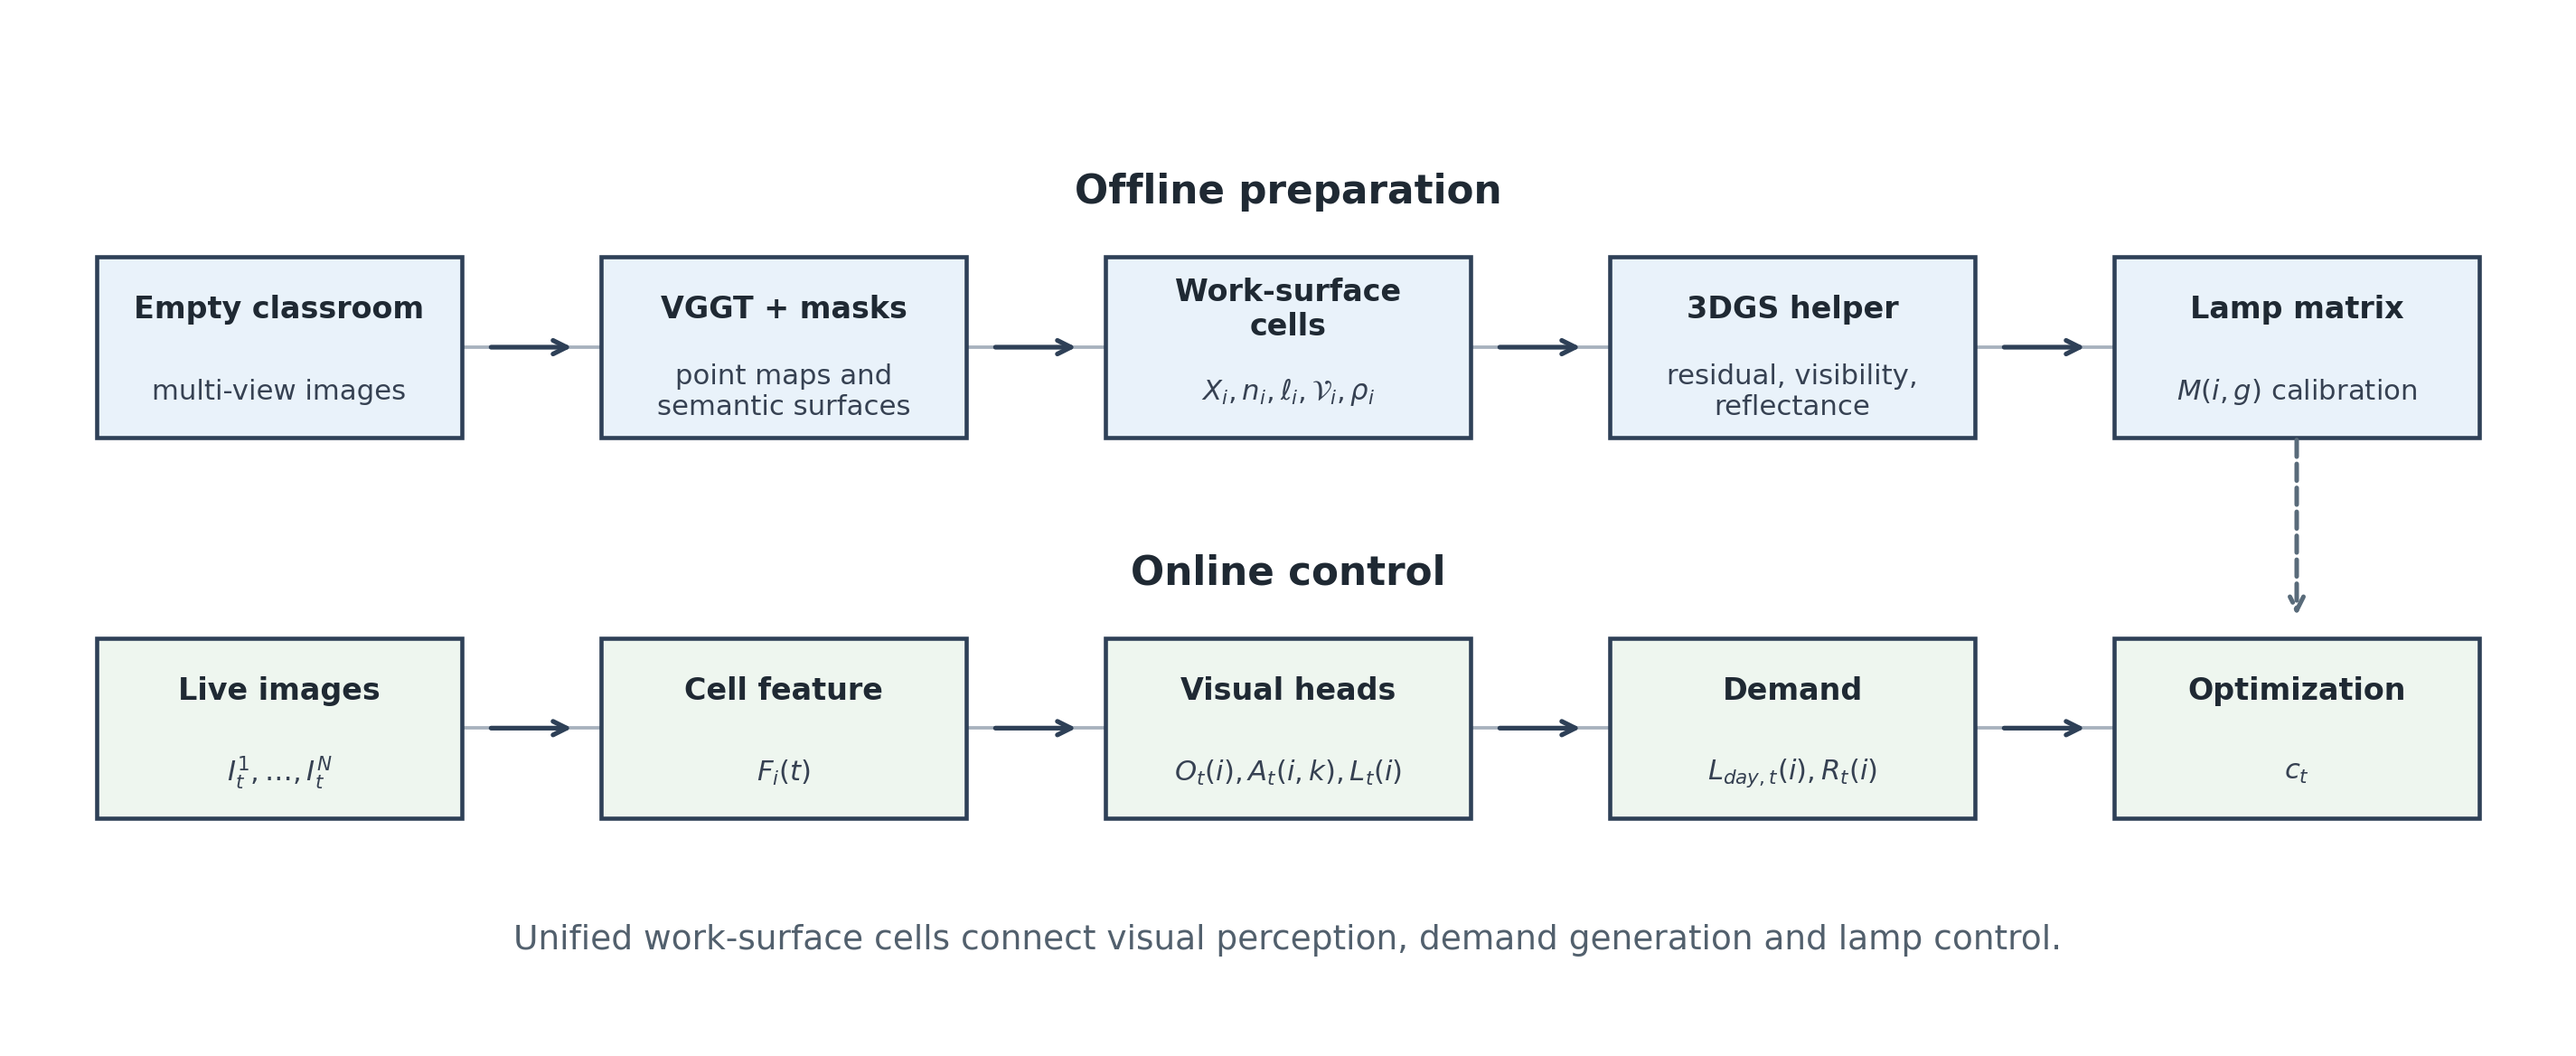
\includegraphics[width=\linewidth]{method_flow.png}
  \caption{纯视觉教室精细照明调控方法总体流程。}
  \label{fig:method-flow}
\end{figure}

\subsection{离线阶段：三维工作表面构建}

\subsubsection{使用 VGGT 点图恢复空教室几何}

离线建模阶段只使用空教室多相机图像。设多个固定相机拍摄的空教室图像为
\begin{equation}
I^1,I^2,\ldots,I^N .
\end{equation}
将这些图像输入 VGGT，得到每个相机的几何信息和点图：
\begin{equation}
\left(K_j,R_j,t_j,P_j\right),\quad j=1,\ldots,N .
\end{equation}
其中，$K_j$ 表示第 $j$ 个相机的内参，$R_j,t_j$ 表示第 $j$ 个相机的外参，$P_j(u)$ 表示第 $j$ 个相机图像中像素 $u$ 对应的三维点。这里最关键的是点图 $P_j$：它将二维图像像素与真实教室三维空间建立了对应关系。后续工作表面提取直接在 VGGT 输出的稠密点图上完成。

\subsubsection{语义掩码与三维语义点集生成}

VGGT 点图只提供几何点，并不知道哪些点属于课桌、黑板或投影幕等对视觉产生主要影响的物体的表面。因此，本文采用“分割模型初分割 + 人工校正关键帧”的方式获得语义掩码，具体分割模型可采用 Mask R-CNN 等实例分割框架\cite{he2017mask}。对第 $j$ 个相机图像，记类别 $c$ 的语义掩码为 $S_j^c(u)$。语义类别固定为
\begin{equation}
c \in \{student\_desk, teacher\_desk, board, screen, aisle, podium, lamp\}.
\end{equation}
若像素 $u$ 在第 $j$ 个图像中属于类别 $c$，即 $S_j^c(u)=1$，则将 VGGT 点图中的三维点 $P_j(u)$ 加入该类别的三维点集：
\begin{equation}
\mathcal{P}_c=\{P_j(u)\mid S_j^c(u)=1,\ j=1,\ldots,N\}.
\end{equation}
由此得到课桌、讲台、黑板、投影幕、过道、教师讲授活动区域和灯具的三维语义点集。该步骤的本质是把二维语义分割结果通过 VGGT 点图提升到三维空间。

\subsubsection{RANSAC 与最小二乘拟合工作表面}

三维语义点集仍然包含分割误差、深度噪声、边界漂移和离群点。对于黑板、投影幕、讲台面、过道地面等近似平面结构，本文采用 RANSAC 剔除离群点，再使用最小二乘精修平面的策略。

对于类别 $c$ 的三维点集 $\mathcal{P}_c$，RANSAC 首先随机采样三点生成候选平面，并以点到平面的距离阈值筛选内点。经过多轮采样后，选择内点数量最多的候选平面。设得到的内点集合为 $\mathcal{I}_c$，则在内点集合上求解最小二乘问题：
\begin{equation}
\min_{n_c,b_c}\sum_{X\in\mathcal{I}_c}\left(n_c^\top X+b_c\right)^2 ,
\end{equation}
并得到最终平面
\begin{equation}
\pi_c:\quad n_c^\top X+b_c=0 .
\end{equation}
其中，$n_c$ 是表面法向，$b_c$ 是平面偏置，$X$ 是三维空间点。对于学生课桌面，不能把所有桌面点拟合成一个整体平面，因为教室中存在多张桌子。本文固定采用高度阈值、DBSCAN 聚类和人工校核的流程，使每个桌面实例分别拟合局部平面。

\subsubsection{工作表面离散化与 cell 属性表}

连续工作表面不能直接用于控制优化，因此需要离散化。本文将所有工作表面离散为三维工作表面单元集合：
\begin{equation}
\mathcal{C}=\{cell_i\}_{i=1}^{S_c}.
\end{equation}
每个 $cell_i$ 是真实物理表面上的一个小区域，既不是图像像素，也不是普通二维 BEV 网格。每个单元保存如下属性：
\begin{equation}
cell_i=\{X_i,n_i,\mathcal{l}_i,\mathcal{V}_i,\rho_i\}.
\end{equation}
其中，$X_i$ 表示单元中心的三维坐标，$n_i$ 表示表面法向，$\mathcal{l}_i$ 表示语义标签，$\mathcal{V}_i$ 表示可以看到该单元的相机集合，$\rho_i$ 表示基础反射外观。后续所有状态量都以 $cell_i$ 为统一索引，包括 $O_t(i)$、$A_t(i,k)$、$L_t(i)$、$L_{day,t}(i)$、$R_t(i)$ 和 $M(i,g)$。图 \ref{fig:cell-distribution} 展示了原型仿真中工作表面 cell 的空间和语义分布。

\begin{figure}[H]
  \centering
  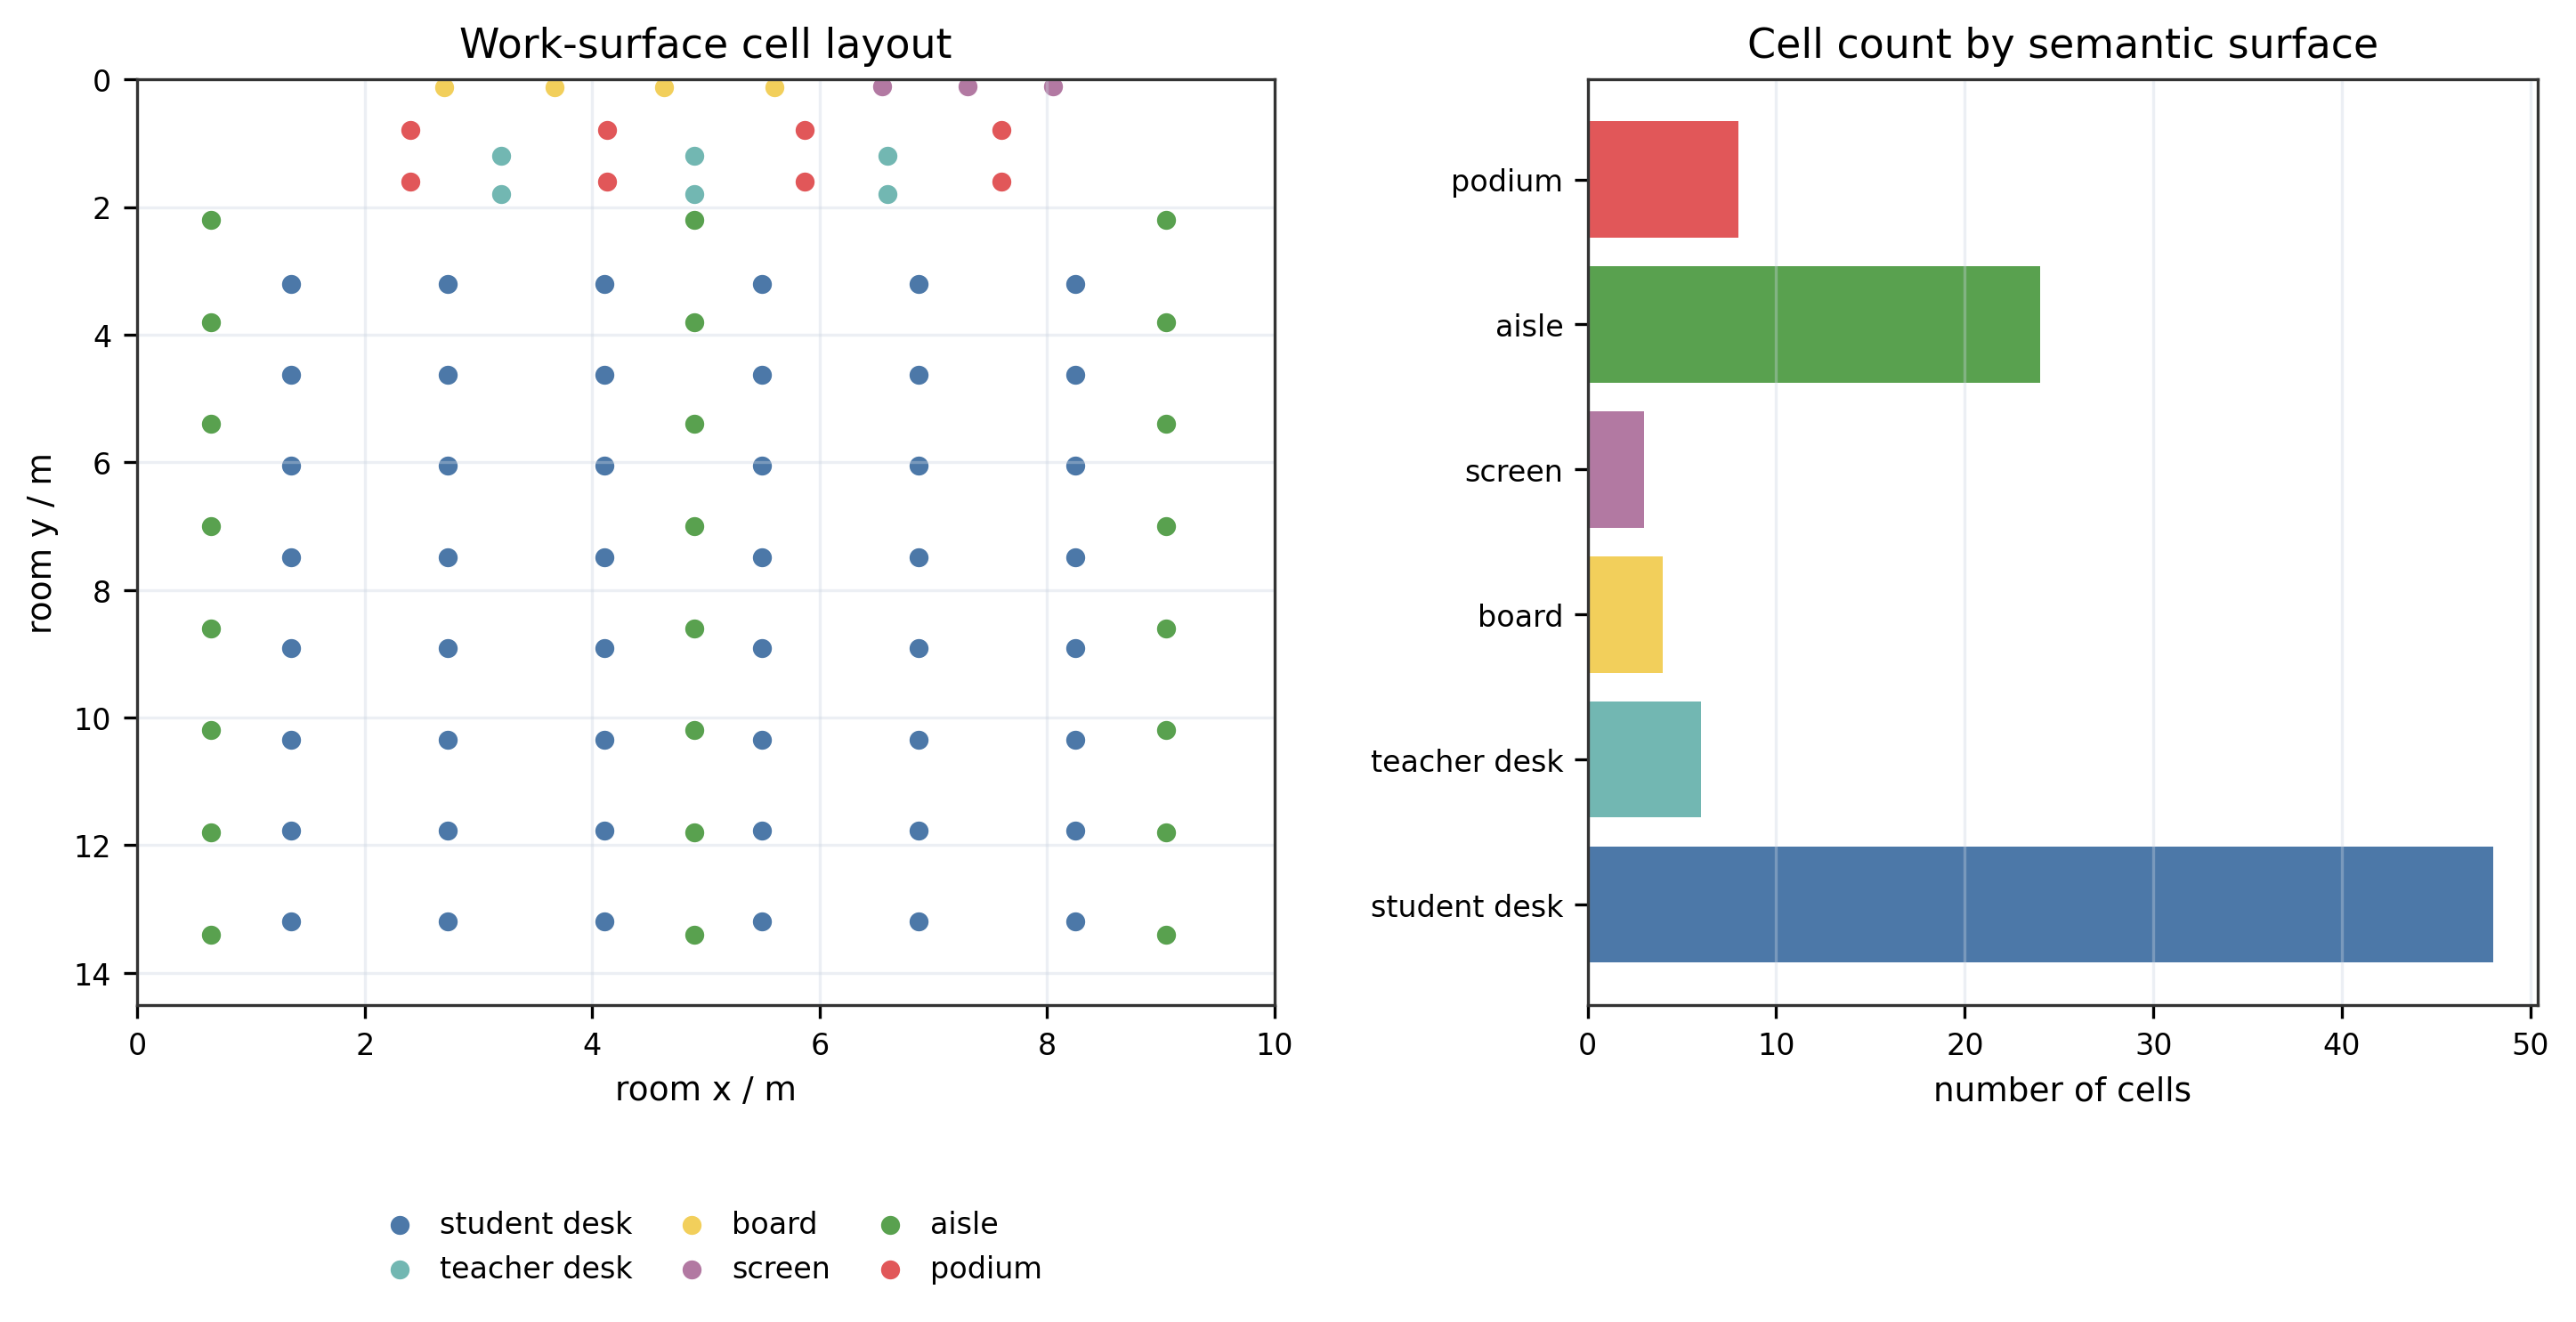
\includegraphics[width=\linewidth]{cell_semantic_distribution.png}
  \caption{工作表面 cell 的语义分布与数量统计。}
  \label{fig:cell-distribution}
\end{figure}

\subsection{3DGS 的定位：静态外观和可见性辅助}

3DGS 的原始表示是一组三维 Gaussian：
\begin{equation}
G_k=\{\mu_k,\Sigma_k,\alpha_k,s_k\}.
\end{equation}
其中，$\mu_k$ 是 Gaussian 中心，$\Sigma_k$ 是协方差，$\alpha_k$ 是不透明度，$s_k$ 是颜色或球谐系数。由于这些 Gaussian 图元和 VGGT 输出的点图相比不适合课桌面、黑板面等表面的提取和重建，因此本文不从 3DGS 中直接提取工作表面。

3DGS 作用主要包括三点。第一，提供静态背景参照：系统优先使用真实空教室背景图像，当视角缺失或需要补全时，利用 3DGS 渲染空教室参考图像，并与当前图像相减生成动态残差，用于突出人员、物体和局部光照变化。第二，辅助多视角可见性判断：3DGS 渲染过程中的 alpha 累积和渲染深度可用于判断 $cell_i$ 在某一相机视角下是否被遮挡，或其投影深度是否一致，从而调整多视角特征融合权重。第三，辅助估计基础反射外观：系统可在真实空教室图像或 3DGS 渲染图像中采样 $cell_i$ 的静态颜色和亮度，得到 $\rho_i$，用于后续光照估计中的表面外观校正。

\subsection{灯具贡献矩阵 M(i,g) 的标定}

灯具贡献矩阵 $M(i,g)$ 表示第 $g$ 组灯在满亮状态下对第 $i$ 个工作表面单元的归一化光照贡献。它是从灯具控制空间到工作表面光照空间的映射。

本文采用空教室灯光切换实验标定 $M$。实验固定包括全关灯、单灯组逐个开启和若干随机灯光组合。设第 $k$ 次实验的灯光控制向量为
\begin{equation}
c^k=\left[c^k(1),c^k(2),\ldots,c^k(G)\right],
\end{equation}
第 $i$ 个工作表面单元在该实验状态下的归一化视觉亮度为 $L^k(i)$，全关灯背景亮度为 $B(i)$，则观测模型为
\begin{equation}
L^k(i)\approx B(i)+\sum_{g=1}^{G}M(i,g)c^k(g).
\end{equation}
学习 $M$ 时使用梯度下降优化完整损失：
\begin{equation}
\mathcal{L}_M=\mathcal{L}_{rec}+\lambda_1\mathcal{L}_{nonneg}+\lambda_2\mathcal{L}_{smooth}+\lambda_3\mathcal{L}_{sparse}+\lambda_4\mathcal{L}_{geo}.
\end{equation}
其中，$\mathcal{L}_{rec}$ 约束由 $M$ 和 $c^k$ 预测的亮度接近观测亮度；$\mathcal{L}_{nonneg}$ 保证灯光贡献非负；$\mathcal{L}_{smooth}$ 约束同一灯组对相邻工作表面的影响连续变化；$\mathcal{L}_{sparse}$ 鼓励每组灯主要影响附近区域；$\mathcal{L}_{geo}$ 使学习结果与由灯具位置、距离衰减、入射角和遮挡关系得到的几何先验保持一致。标定完成后，$M$ 作为系统参数固定下来。图 \ref{fig:contribution-matrix} 给出了原型中的归一化贡献矩阵。

\begin{figure}[H]
  \centering
  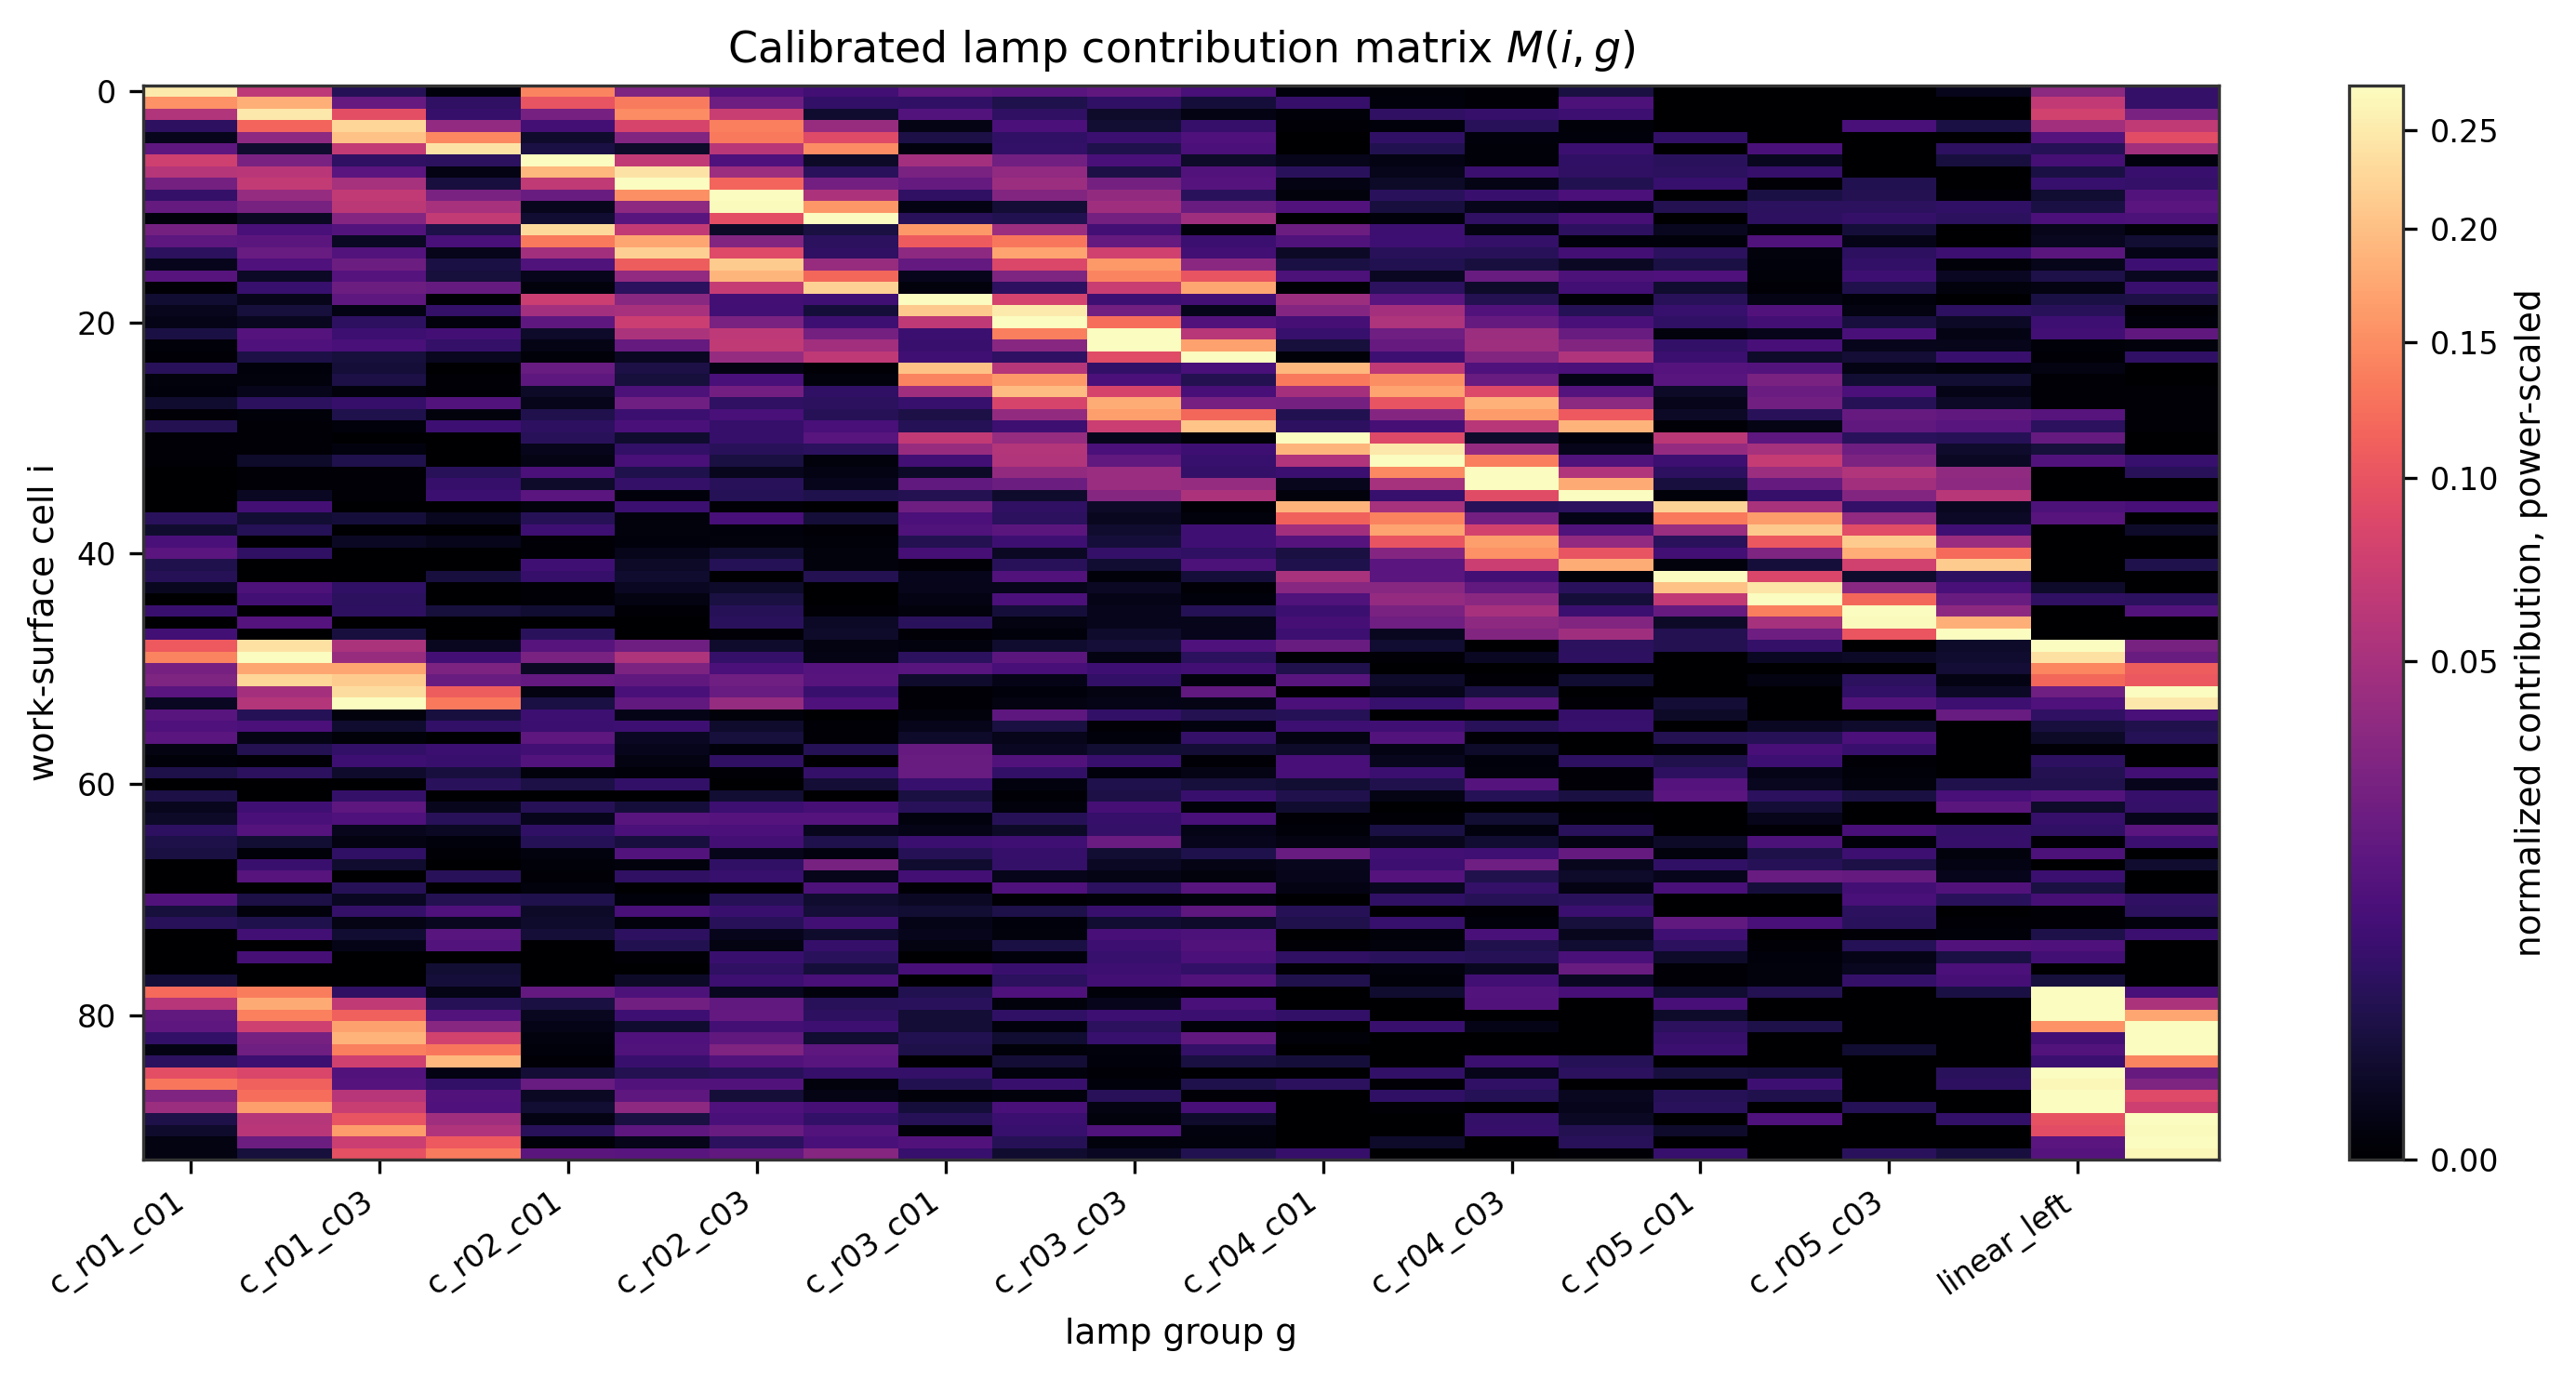
\includegraphics[width=\linewidth]{contribution_matrix.png}
  \caption{灯具贡献矩阵 $M(i,g)$ 的原型标定结果。}
  \label{fig:contribution-matrix}
\end{figure}

\subsection{在线视觉感知：Swin-Tiny-FPN 与三任务 head}

\subsubsection{多相机图像特征提取}

在线时刻 $t$，输入实时多相机图像 $I_t^1,I_t^2,\ldots,I_t^N$。每个图像经过共享视觉 backbone：
\begin{equation}
F_t^j=\Phi(I_t^j).
\end{equation}
本文将 $\Phi$ 具体设置为 Swin-Tiny-FPN。Swin-Tiny 通过 shifted window 注意力提取层级视觉特征，FPN 对不同层级特征进行自顶向下融合，形成适合多尺度 cell 投影采样的特征图。该 backbone 使用预训练权重初始化，训练时使用教室数据调整占用、活动和光照三个任务分支，并可参考多任务学习中的不确定性加权思想平衡不同 head 的训练目标\cite{kendall2018multitask}。注意，这里的 backbone 负责提取通用视觉特征，最终状态不是由 backbone 直接输出，而是由后续三个任务 head 输出。

\subsubsection{多视角特征融合到 cell}

对于每个 $cell_i$，已知其三维中心 $X_i$。通过第 $j$ 个相机的投影函数，计算
\begin{equation}
u_{ij}=\Pi_j(X_i).
\end{equation}
然后在第 $j$ 个相机的多尺度特征图中采样局部特征。由于 FPN 提供多个尺度，本文根据 $cell_i$ 投影区域的尺度选择对应层级，或对相邻层级进行加权融合：
\begin{equation}
f_{ij}(t)=Sample(\{F_{t,l}^{j}\}_{l=1}^{L},u_{ij}).
\end{equation}
多个相机的观测加权融合为
\begin{equation}
\bar{f}_i(t)=\sum_{j=1}^{N}w_{ij}(t)f_{ij}(t),
\end{equation}
其中，$w_{ij}(t)$ 由可见性、视角质量和遮挡状态决定。与将多相机特征直接提升到 BEV 的方法\cite{liang2020lift,li2022bevformer}不同，本文将特征组织到真实三维工作表面 cell 上。再将动态视觉特征与静态空间先验融合：
\begin{equation}
s_i=E_S(X_i,n_i,\mathcal{l}_i,\rho_i,\mathcal{V}_i).
\end{equation}
结合动态残差特征 $\Delta\bar{f}_i(t)$，得到
\begin{equation}
F_i(t)=\phi_{fuse}\left([\bar{f}_i(t),s_i,\Delta\bar{f}_i(t)]\right).
\end{equation}
这里 $F_i(t)$ 是 $cell_i$ 的融合观测特征，不是最终状态。最终的人员占用、活动状态和当前光照分别由三个任务 head 输出。

\subsubsection{占用、活动与光照 head}

occupancy head 直接接收 $F_i(t)$ 并输出人员占用概率：
\begin{equation}
O_t(i)=h_{occ}(F_i(t)),\quad O_t(i)\in[0,1].
\end{equation}
$O_t(i)$ 表示与 $cell_i$ 相关联的人员活动邻域中是否有人，而不是“人是否站在 $cell_i$ 表面上”。例如，学生课桌 cell 的占用标签由其对应座位区域是否有人决定；过道 cell 的占用标签由其上方通行区域是否有人决定；讲台 cell 的占用标签由教师活动区域是否有人决定。

activity head 输出每个 $cell_i$ 的活动状态概率：
\begin{equation}
A_t(i,k)=h_{act}(F_i(t),O_t(i),\mathcal{l}_i,T_i(t)).
\end{equation}
其中，$T_i(t)$ 表示 cell 级别的时序特征，可由过去若干帧的 $F_i(t)$、$O_t(i)$ 或隐藏状态构成。活动类别固定为
\begin{equation}
k\in\{empty,listening,writing,projection,blackboard\text{-}writing,discussion,walking\},
\end{equation}
且满足 $\sum_k A_t(i,k)=1$。活动状态不再依赖显式人体轨迹，而是依赖 cell 级观测特征、占用概率、语义标签和时序变化。

lighting head 输出当前归一化视觉照明量：
\begin{equation}
L_t(i)=h_{light}(F_i(t),\rho_i,\mathcal{l}_i),\quad L_t(i)\in[0,1].
\end{equation}
由于本文纯视觉不使用照度计，$L_t(i)$ 表示工作表面在视觉上的归一化亮度状态。光照 head 使用小型 MLP 实现，输入包括融合观测特征、基础反射外观和表面语义信息。光照 head 的无标定训练损失为
\begin{equation}
\mathcal{L}_{light}=\lambda_p\mathcal{L}_{photo}+\lambda_m\mathcal{L}_{mv}+\lambda_s\mathcal{L}_{smooth}.
\end{equation}

\subsection{环境光分离}

当前光照 $L_t(i)$ 包含不可控环境光和上一时刻人工灯光贡献。利用已标定的灯光贡献矩阵 $M(i,g)$ 和上一时刻控制量 $c_{t-1}(g)$，可写为
\begin{equation}
L_t(i)=L_{day,t}(i)+\sum_{g=1}^{G}M(i,g)c_{t-1}(g).
\end{equation}
因此
\begin{equation}
L_{day,t}(i)=\max\left(0,L_t(i)-\sum_{g=1}^{G}M(i,g)c_{t-1}(g)\right).
\end{equation}
这里的 $L_{day,t}(i)$ 表示除可控灯具贡献之外的不可控背景光，包括自然光、室外反射光和其他不可控光源。

\subsection{目标照明需求生成与可学习需求系数}

目标照明需求 $R_t(i)$ 表示第 $i$ 个工作表面单元当前应达到的归一化视觉亮度。由于不使用照度计，本文使用的是归一化目标值，例如 0.3、0.6、0.8。目标需求由基础项、占用项和活动项组成：
\begin{equation}
R_t(i)=R_{base}(i)+R_{occ}(i)+R_{act}(i).
\end{equation}
基础项由表面语义决定：
\begin{equation}
R_{base}(i)=b_{\mathcal{l}_i}.
\end{equation}
占用项由 occupancy head 输出决定：
\begin{equation}
R_{occ}(i)=\lambda_{\mathcal{l}_i}^{occ}O_t(i).
\end{equation}
活动项为
\begin{equation}
R_{act}(i)=O_t(i)\sum_k A_t(i,k)r_{\mathcal{l}_i,k}+\mathbf{1}[i\in\Omega_{board}]s_{board,t}r_{board}.
\end{equation}
其中
\begin{equation}
s_{board,t}=\max_{q\in\Omega_{board\_front}}A_t(q,blackboard\text{-}writing).
\end{equation}
第一项表示当前 cell 附近有人并发生某种活动时产生的本地活动需求。第二项是黑板板书传播项：当黑板前区域检测到板书活动时，黑板面作为被观看和书写的任务表面，需要提高照明需求。该项只作用于 $\Omega_{board}$ 中的黑板 cell，不影响课桌、过道或投影幕等工作表面。

需求函数中的策略系数记为
\begin{equation}
\theta_R=\{b_{\mathcal{l}},\lambda_{\mathcal{l}}^{occ},r_{\mathcal{l},k},r_{board}\}.
\end{equation}
这些系数不再完全由人工设定，而是通过人工标注的最终灯光控制策略进行离线校准。对于若干典型课堂场景，由人工给出期望灯光控制向量
\begin{equation}
c_t^{gt}=[c_t^{gt}(1),c_t^{gt}(2),\ldots,c_t^{gt}(G)].
\end{equation}
需求系数首先生成 $R_t(i;\theta_R)$，目标需求进入控制代价函数并经过可微展开控制层输出预测控制向量 $\widehat{c}_t$。训练损失为
\begin{equation}
\mathcal{L}_R=\lambda_c\|\widehat{c}_t-c_t^{gt}\|_2^2+\lambda_l\|L_{pred}(\widehat{c}_t)-L_{pred}(c_t^{gt})\|_2^2+\lambda_p\|\theta_R-\theta_R^0\|_2^2 .
\end{equation}
为了使梯度能够从人工控制策略误差传回需求系数，训练阶段将控制求解展开为 $K$ 步可微投影梯度迭代。设 $\widehat{c}_t^{(0)}=c_{t-1}$，第 $r$ 步更新为
\begin{equation}
\widehat{c}_t^{(r+1)}=\Pi_{[0,1]}\left(\widehat{c}_t^{(r)}-\tau\nabla_cJ(\widehat{c}_t^{(r)};R_t(\theta_R),L_{day,t},M)\right),\quad r=0,\ldots,K-1.
\end{equation}
经过 $K$ 步后得到 $\widehat{c}_t=\widehat{c}_t^{(K)}$。在线阶段则固定校准后的 $\theta_R$，不再更新需求系数。

\subsection{控制优化}

控制器输入包括环境光 $L_{day,t}(i)$、目标需求 $R_t(i)$、亮度上限 $R_{high,t}(i)$、灯光贡献矩阵 $M(i,g)$ 和上一时刻灯光状态 $c_{t-1}$。控制器要求解当前灯光控制向量
\begin{equation}
c_t=[c_t(1),c_t(2),\ldots,c_t(G)],\quad 0\leq c_t(g)\leq 1.
\end{equation}
给定候选控制向量 $c_t$，预测工作表面亮度为
\begin{equation}
L_{pred}(i,c_t)=L_{day,t}(i)+\sum_{g=1}^{G}M(i,g)c_t(g).
\end{equation}
控制代价函数定义为
\begin{equation}
J(c_t)=\alpha E(c_t)+\beta U(c_t)+\gamma O(c_t)+\delta S(c_t)+\eta F(c_t).
\end{equation}
其中，$E(c_t)$ 为能耗项，$U(c_t)$ 为欠照惩罚，$O(c_t)$ 为过照惩罚，$S(c_t)$ 为调光平滑项，$F(c_t)$ 为局部均匀性项。欠照惩罚约束重要工作表面达到目标需求，过照惩罚限制投影幕等区域过亮，平滑项避免灯光突变，局部均匀性项减少活动区域内部亮度差异。

在线控制时，需求系数 $\theta_R$ 已在离线训练阶段校准完成，因此 $R_t(i)$ 被视为当前场景下的已知目标需求。求解时采用 L-BFGS-B。初始点取上一时刻灯光状态 $c_t^{(0)}=c_{t-1}$。优化器根据 $J(c_t)$ 对 $c_t$ 的梯度迭代更新，并在边界约束下求得近似最优控制向量：
\begin{equation}
c_t^*=\arg\min_{0\leq c_t\leq 1}J(c_t).
\end{equation}
如果实际灯具只支持离散档位，则先求连续解，再将结果量化到最近档位。需要强调的是，控制优化不是训练神经网络，其优化对象是当前灯光控制向量 $c_t$，不是模型参数。

\subsection{训练、标定、需求系数校准与在线控制的区分}

本文中存在四类不同的优化过程，它们的优化对象不同。第一类是视觉感知网络调整。Swin-Tiny-FPN 共享 backbone 使用预训练权重初始化，占用、活动和光照三个任务 head 使用教室数据进行调整，对应损失为
\begin{equation}
\mathcal{L}_{vision}=\lambda_{occ}\mathcal{L}_{occ}+\lambda_{act}\mathcal{L}_{act}+\lambda_{light}\mathcal{L}_{light}.
\end{equation}
这里更新的是视觉网络参数，包括任务 head 参数以及可选的小学习率 backbone 参数，目标是提高 $O_t(i)$、$A_t(i,k)$ 和 $L_t(i)$ 的估计质量。

第二类是离线系统参数标定，包括 3DGS 静态表示优化和灯具贡献矩阵 $M$ 的标定优化。3DGS 优化的是静态 Gaussian 场景参数，$M$ 的标定优化的是灯具到工作表面的贡献矩阵。这些参数在在线控制阶段固定使用。

第三类是需求系数校准。需求系数 $\theta_R$ 决定了感知状态如何转化为目标需求 $R_t(i)$。本文不直接标注逐 cell 目标亮度，而是利用人工控制策略 $c_t^{gt}$ 作为间接监督。校准时先固定视觉感知网络和 $M$，只更新 $\theta_R$，避免需求系数吸收视觉感知误差。校准完成后，$\theta_R$ 固定用于在线目标需求生成。

第四类是在线控制优化。在线阶段不再更新网络参数，也不再更新需求系数，而是使用当前感知状态、已标定的 $M$ 和已校准的 $\theta_R$，通过 L-BFGS-B 求解当前时刻的灯光控制向量 $c_t$。

\section{原型仿真验证与结果分析}

本文定位为方法设计与原型仿真验证。验证重点不是完整工程部署，而是检查方法链条是否闭合、各变量是否能够在统一 $cell_i$ 索引下工作，以及控制优化是否能够根据归一化目标需求给出合理灯光方案。原型仿真程序采用合成点图、合成多相机观测和规则化感知 head，模拟课堂书写、课间讨论、投影、板书和自习五类课堂状态。该验证不使用真实训练权重、真实灯具硬件或照度计，因此结果只表示方法流程和变量关系的可执行性，不代表真实部署性能。真实教室数据采集、硬件接口和长期运行评价不属于本文验证范围。

\begin{table}[H]
  \centering
  \caption{原型仿真输入、场景与输出内容}
  \label{tab:prototype-setting}
  \begin{tabularx}{\linewidth}{>{\raggedright\arraybackslash}p{0.20\linewidth}>{\raggedright\arraybackslash}X}
    \toprule
    项目 & 内容 \\
    \midrule
    输入数据 & 合成 VGGT 点图、合成多相机观测、规则化感知输出；不使用真实多相机采集数据 \\
    工作表面 & 课桌、教师桌、黑板、投影幕、过道和讲台，共 93 个 work-surface cell \\
    灯具控制量 & 20 个顶灯和 2 个前方线性灯组，共 22 个控制变量 \\
    课堂状态 & 课堂书写、课间讨论、投影、板书、自习五类典型状态 \\
    输出变量 & $O_t(i)$、$A_t(i,k)$、$L_t(i)$、$L_{day,t}(i)$、$R_t(i)$、$M(i,g)$、$c_t$ 及欠照/过照指标 \\
    \bottomrule
  \end{tabularx}
\end{table}

原型输出包括工作表面 cell、三任务感知状态、灯具贡献矩阵、目标需求、预测亮度、欠照/过照指标和灯具控制向量。评价指标采用归一化误差和任务满足率，不使用 lux 误差。归一化光照估计误差可写为
\begin{equation}
E_L=\frac{1}{S_c}\sum_{i=1}^{S_c}|L_t(i)-\widehat{L}_t(i)|.
\end{equation}
控制效果主要观察三个方面：一是高需求 cell 的欠照是否保持在较低水平；二是过照是否被亮度上限抑制；三是灯具控制向量的相对能耗估计是否低于全开基线。这里的相对能耗由归一化灯具控制向量估算，不等同于真实电表功耗。

图 \ref{fig:demand-prediction} 对比了不同场景中任务相关 cell 的平均目标需求和优化后的预测亮度。结果显示，优化器并不追求所有 cell 统一高亮，而是根据不同场景的 cell 需求生成差异化照明。class writing 和 projection 场景的目标需求较高，控制结果相应提高预测亮度；break discussion 和 self study 场景中，高需求区域较局部，因此控制量随活动范围变化。欠照指标在任务相关 cell 上保持较低水平，说明当前原型将主要教学活动表面的需求满足作为优先条件，同时仍保留相对全开状态的能耗下降空间。

\begin{figure}[H]
  \centering
  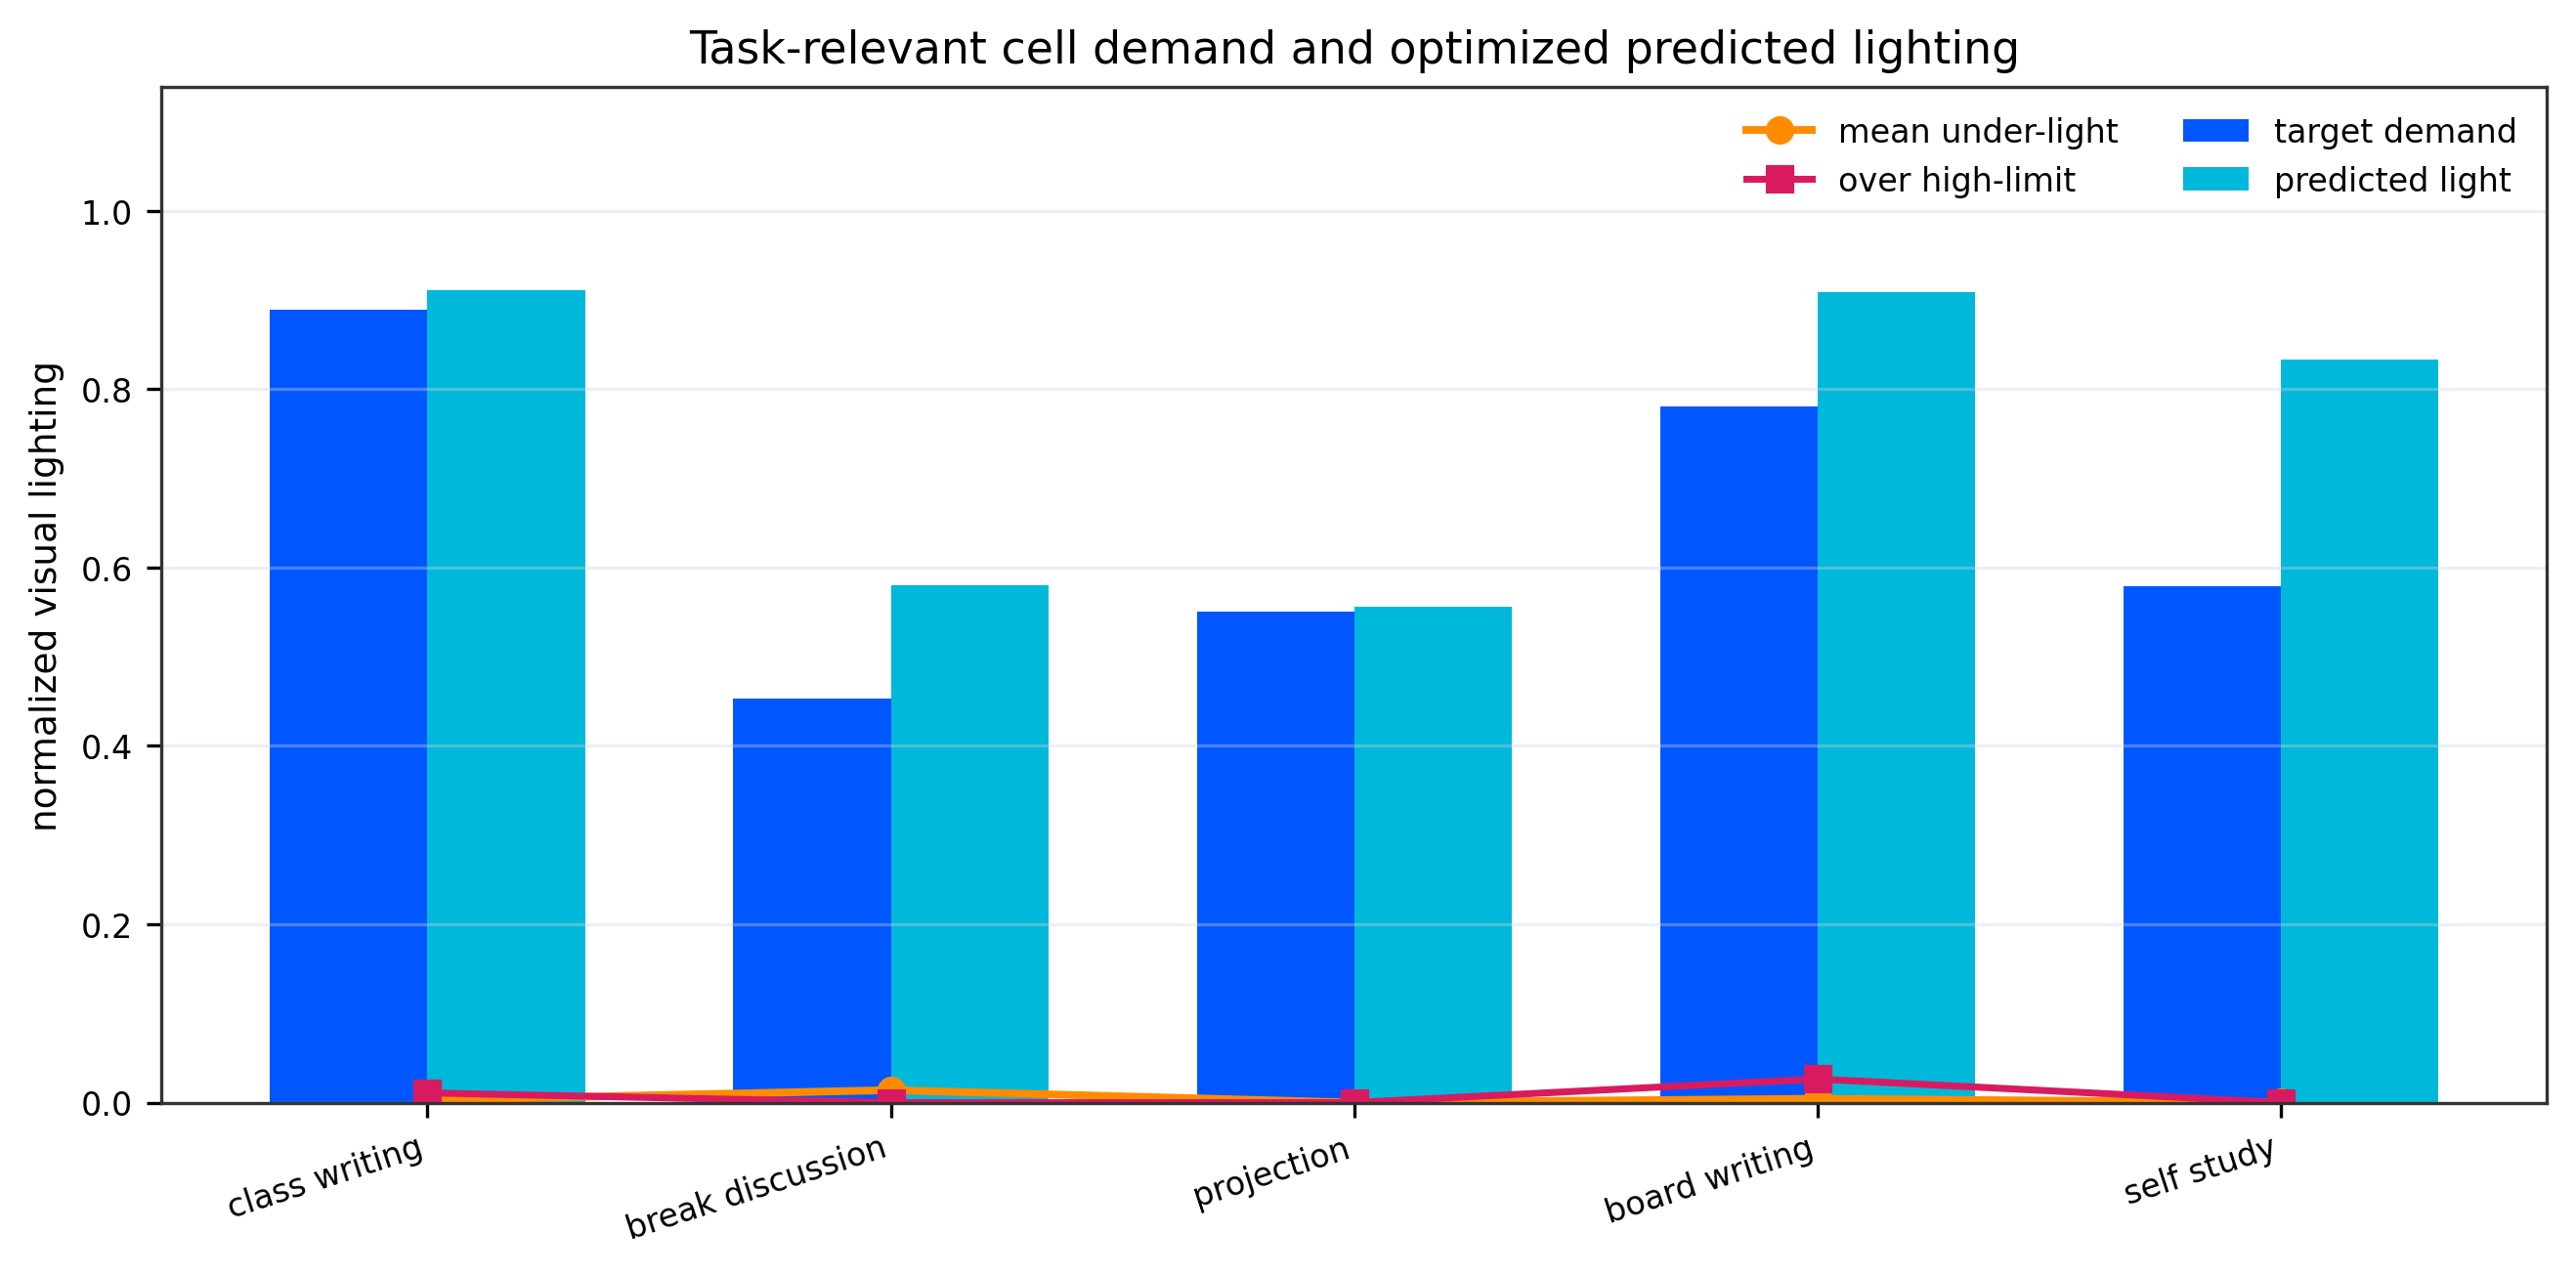
\includegraphics[width=\linewidth]{demand_prediction_by_scenario.png}
  \caption{不同课堂状态下任务相关 cell 的目标需求、预测亮度、欠照与亮度上限过照对比。}
  \label{fig:demand-prediction}
\end{figure}

图 \ref{fig:control-vector} 展示了五类场景下的灯具控制向量 $c_t$。可以看到，不同场景并没有产生相同的灯具亮度模式。书写和板书相关场景需要提高部分工作表面的亮度，投影场景则需要兼顾观看区域与投影幕过亮风险，自习场景中控制量更加局部化。这说明在原型层面，控制向量确实由 cell 级需求和贡献矩阵共同决定，而不是简单的房间级统一调光。

\begin{figure}[H]
  \centering
  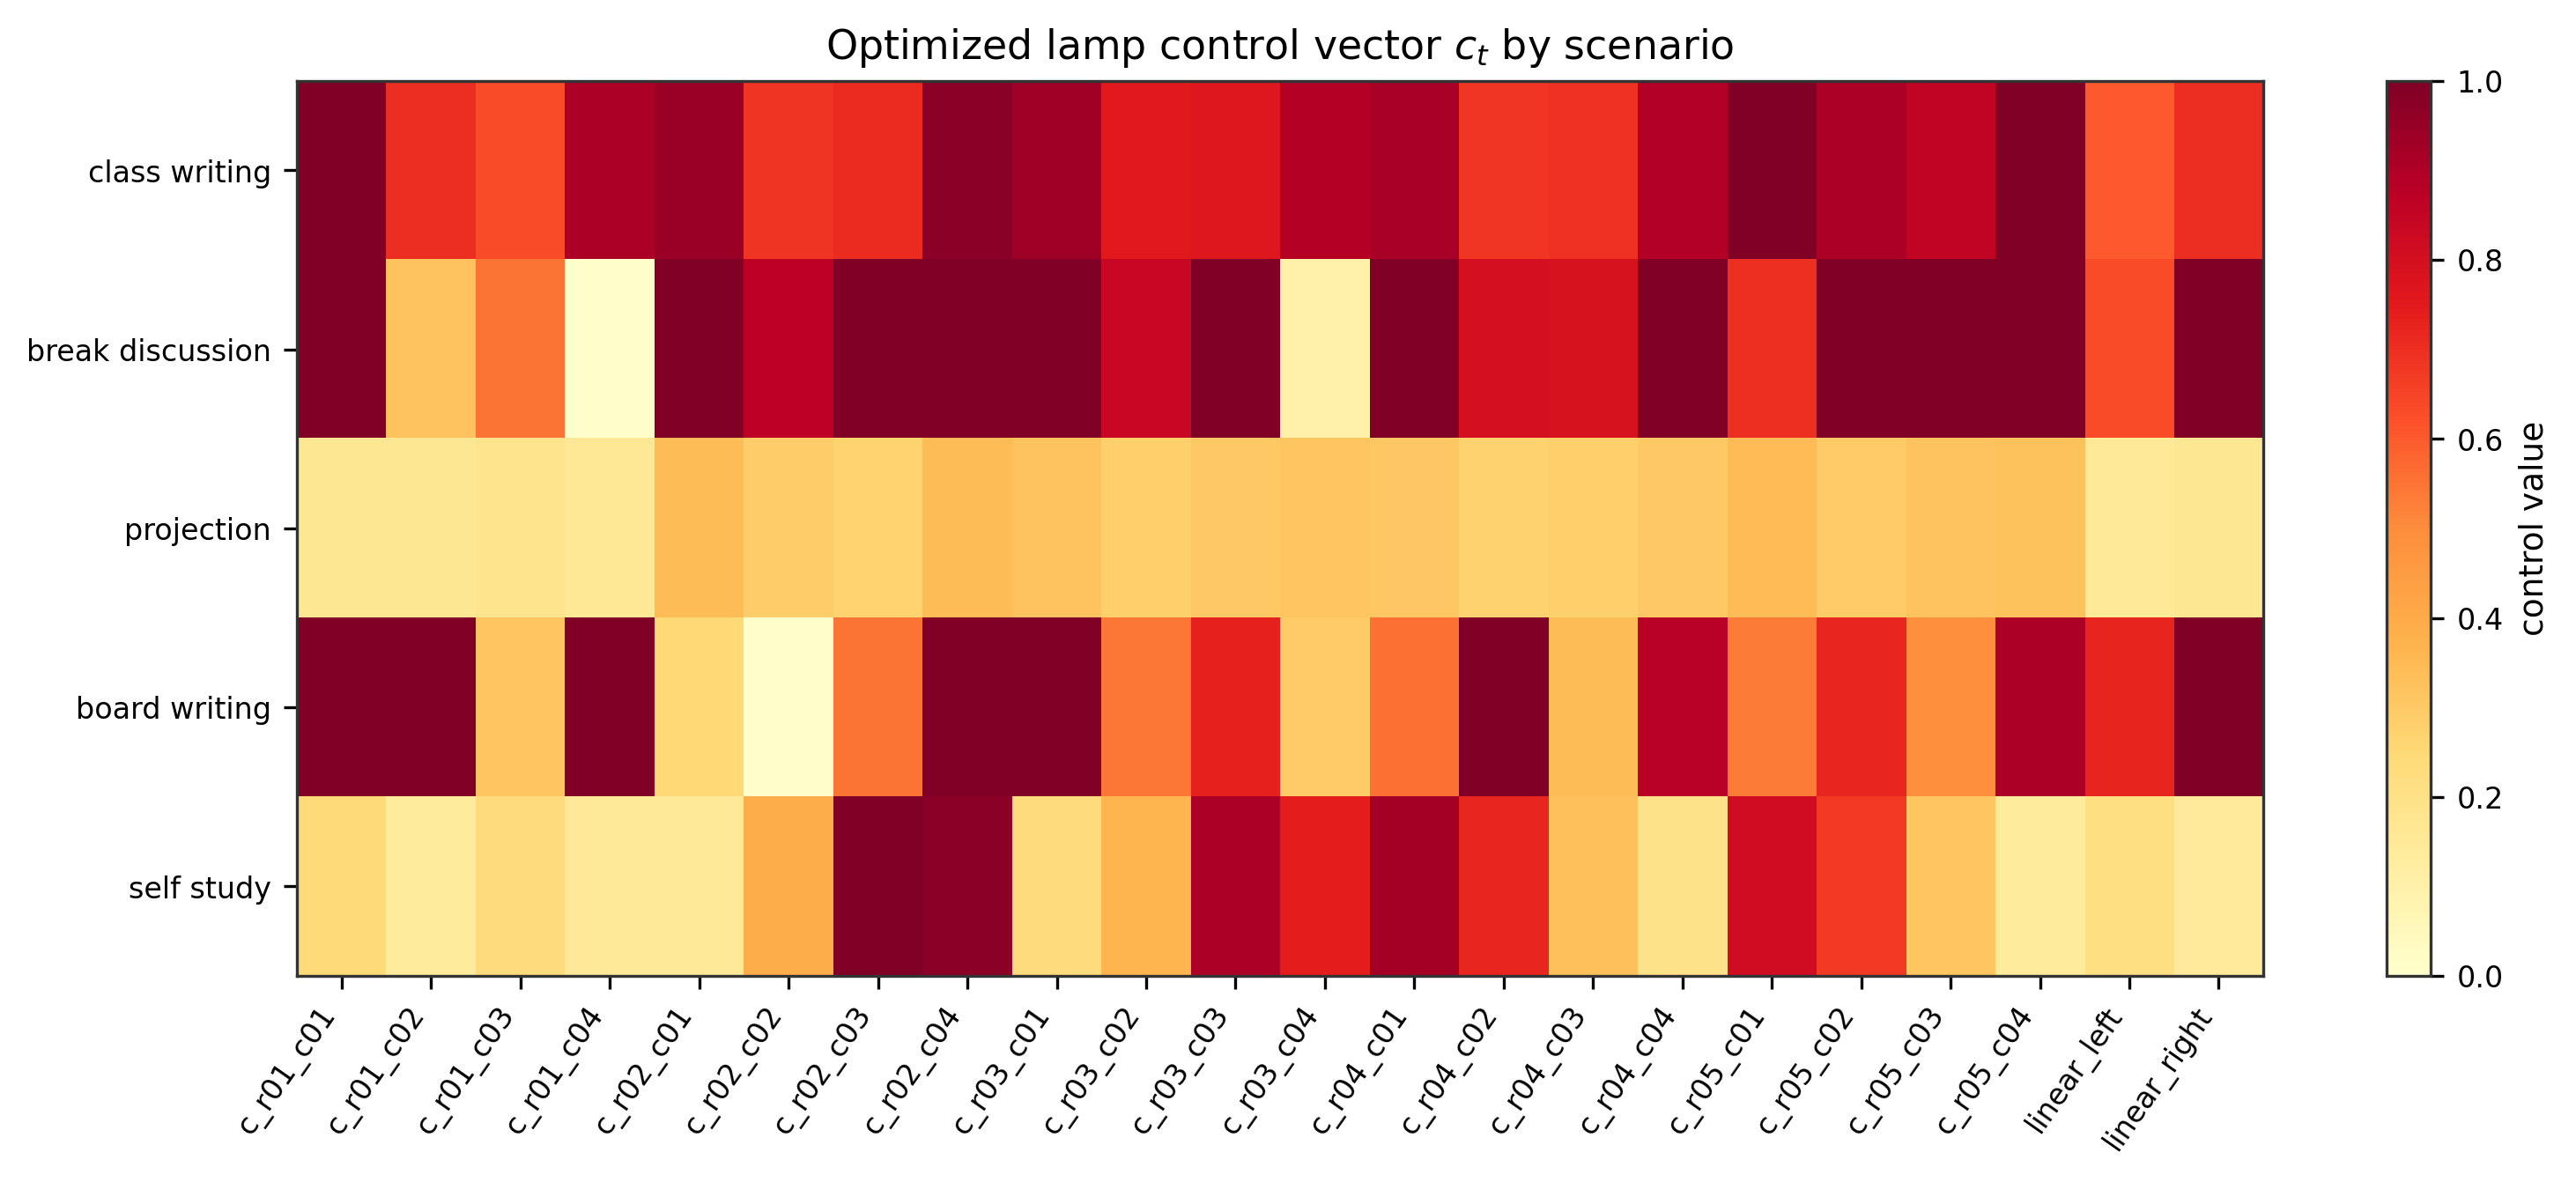
\includegraphics[width=\linewidth]{control_vectors.png}
  \caption{不同课堂状态下的灯具控制向量 $c_t$。}
  \label{fig:control-vector}
\end{figure}

图 \ref{fig:quality-metrics} 汇总了原型仿真中的任务相关欠照、亮度上限过照、相对能耗估计和任务满足率。整体上，五类场景在设定容差内的任务满足率均达到 1.000，任务相关平均欠照保持在较低水平。class writing 场景覆盖课桌、教师桌和讲台等大范围工作表面，相对能耗估计最高，为 0.825；break discussion 场景考虑课间走动、讨论以及可能存在的短时书写需求，相对能耗估计为 0.799，接近上课模式；projection 场景需要降低投影区域强光，相对能耗估计最低；board writing 与 self study 场景分别体现前区板书照明和局部自习照明。该结果符合本文方法的预期：控制器不是单独最大化节能，也不是简单保持全教室高亮，而是在满足任务表面需求的前提下，根据场景活动范围进行相对节能控制。

\begin{figure}[H]
  \centering
  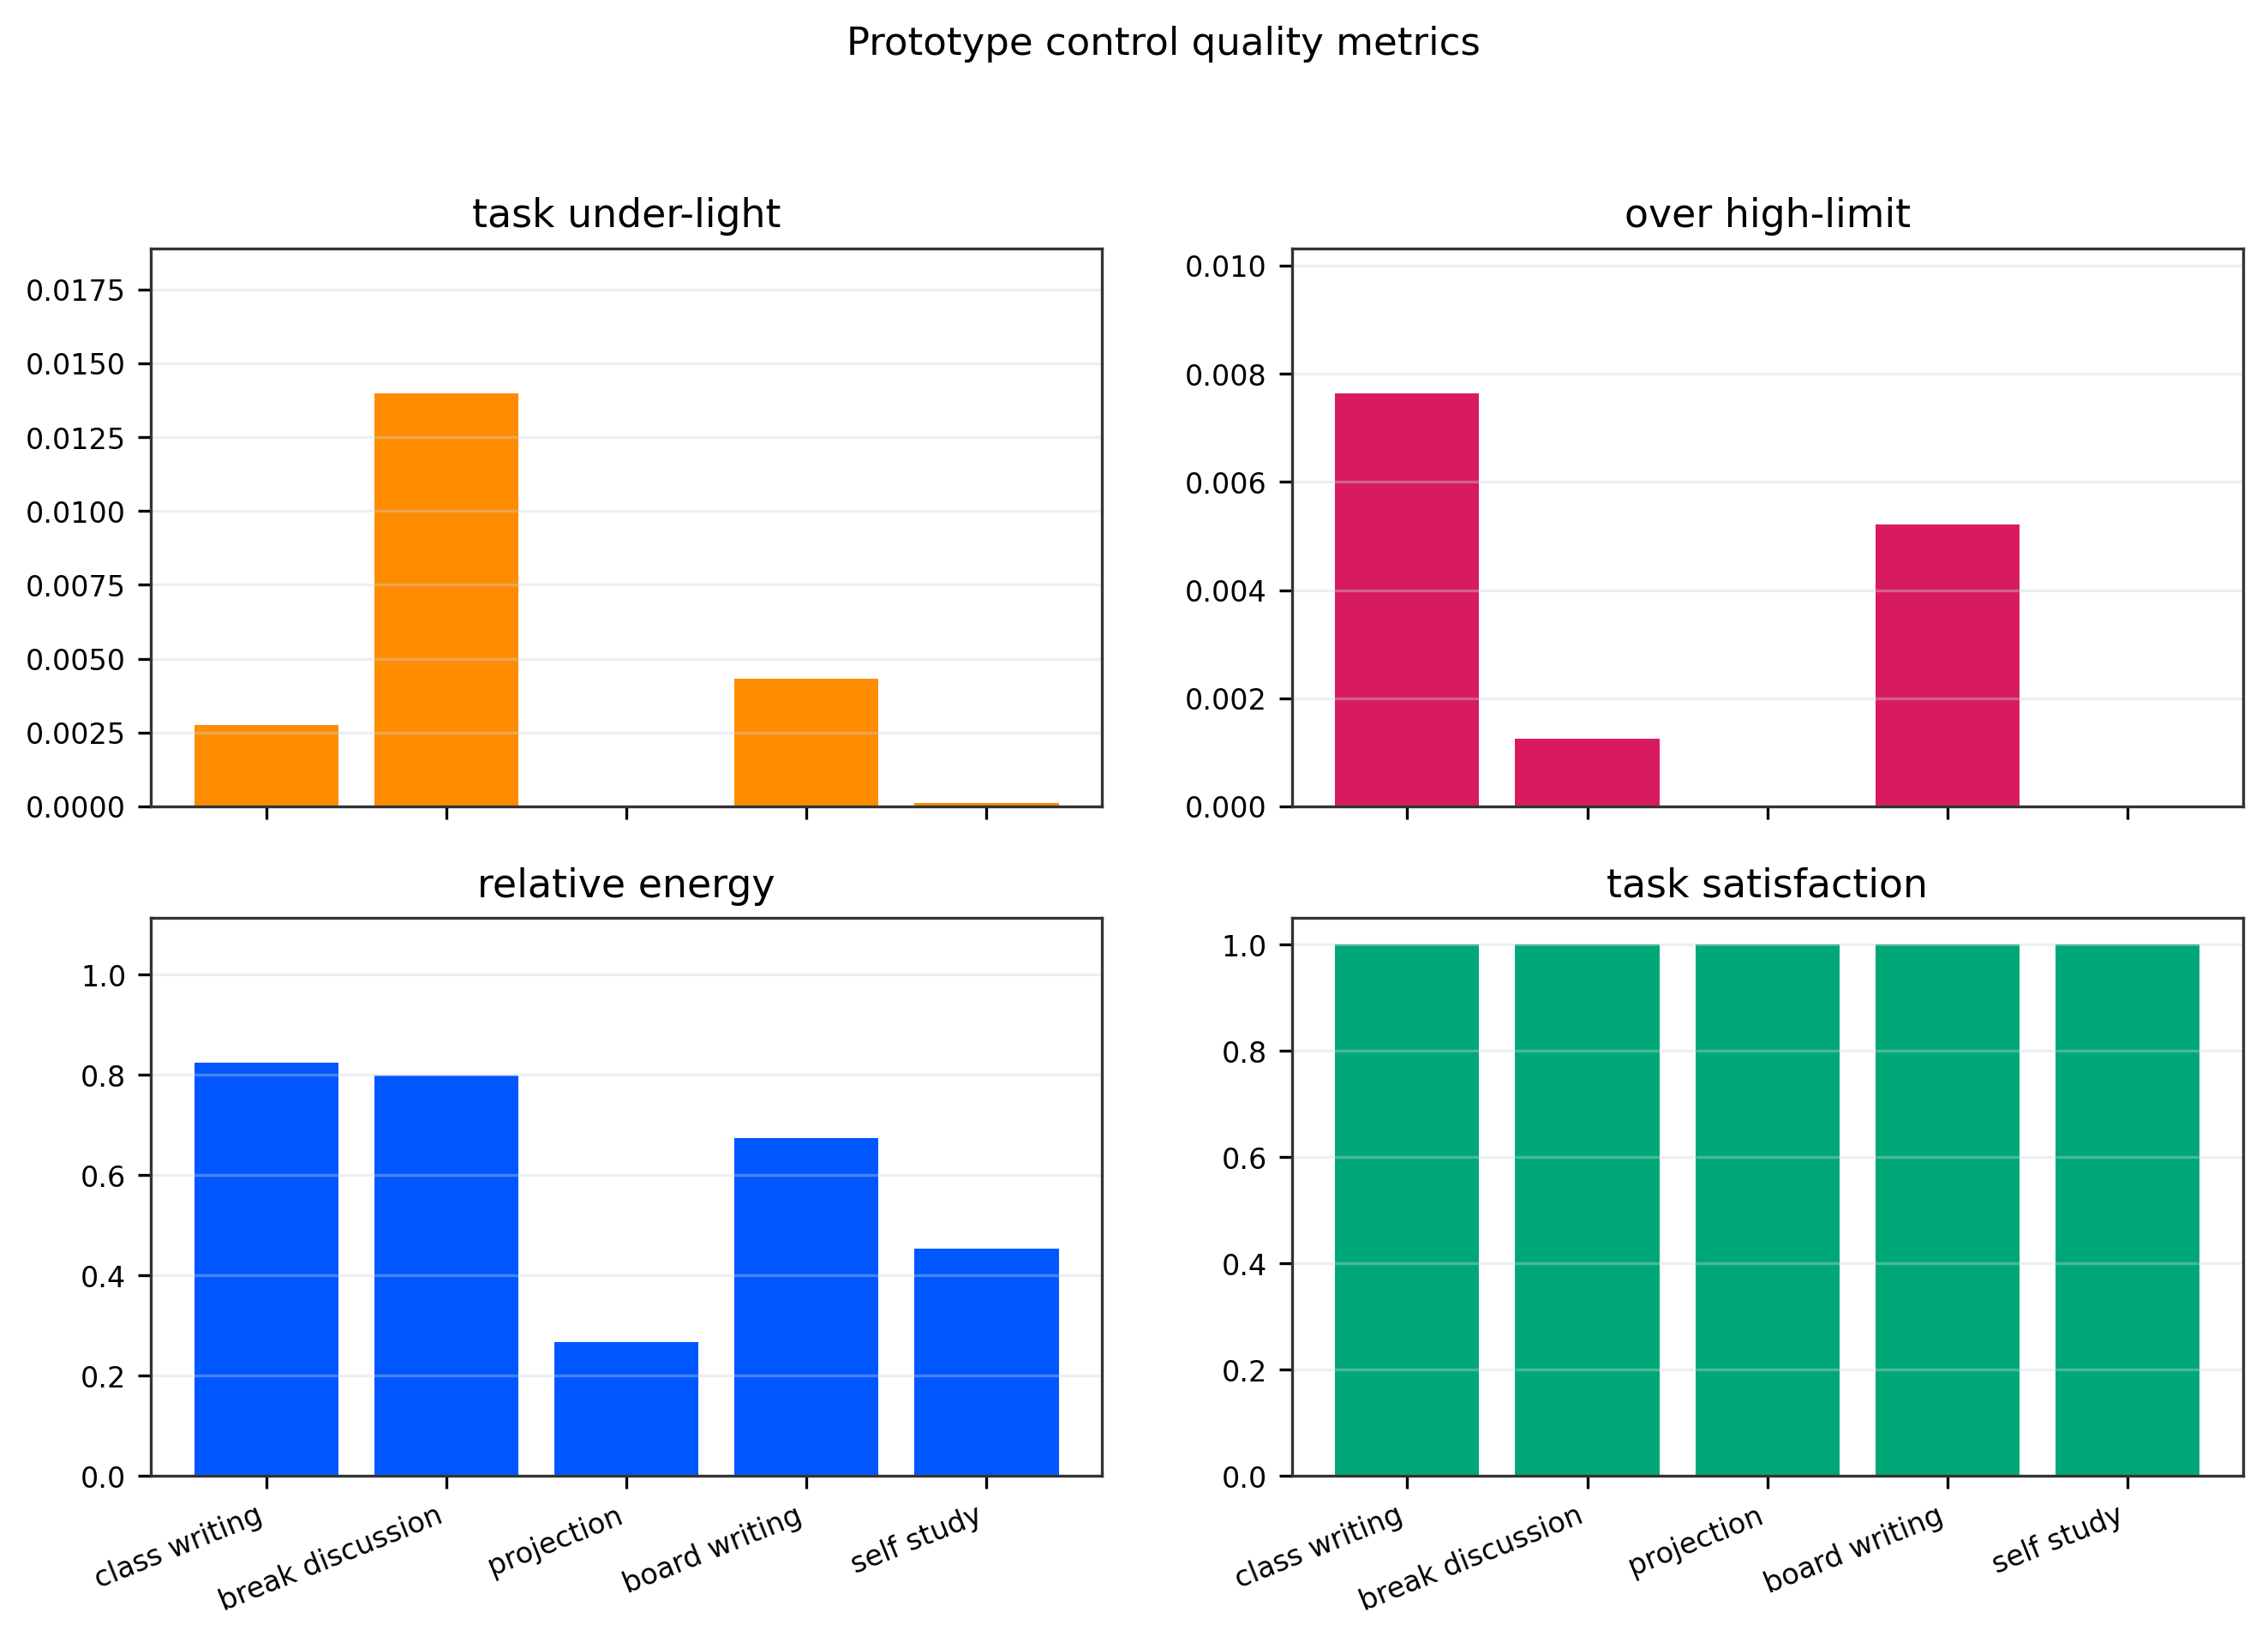
\includegraphics[width=\linewidth]{prototype_quality_metrics.png}
  \caption{原型仿真控制质量指标。}
  \label{fig:quality-metrics}
\end{figure}

\begin{table}[H]
  \centering
  \caption{原型仿真主要质量指标}
  \label{tab:quality-metrics}
  \begin{tabular}{lccccc}
    \toprule
    场景 & 任务欠照 & 上限过照 & 相对能耗 & 任务满足率 & 光照估计误差 \\
    \midrule
    课堂书写 & 0.003 & 0.008 & 0.825 & 1.000 & 0.341 \\
    课间讨论 & 0.014 & 0.001 & 0.799 & 1.000 & 0.339 \\
    投影 & 0.000 & 0.000 & 0.266 & 1.000 & 0.041 \\
    板书 & 0.004 & 0.005 & 0.675 & 1.000 & 0.281 \\
    自习 & 0.000 & 0.000 & 0.454 & 1.000 & 0.134 \\
    \bottomrule
  \end{tabular}
\end{table}

综合来看，原型仿真验证表明，本文提出的变量链路能够在代码层面闭合：工作表面 cell 能够承载占用、活动、当前光照、目标需求和灯具贡献；灯具贡献矩阵能够把控制变量映射到工作表面光照；目标需求函数能够把课堂活动转化为控制目标；约束优化能够输出满足边界约束的灯具控制向量。同时，原型结果也说明，视觉感知精度、真实光照标定、灯具功率曲线、相机遮挡、长期光照变化和用户舒适度反馈等问题不能由当前仿真直接回答，应在独立的工程验证研究中另行评估。

\section{研究结论}

本文围绕绿色低碳校园中的教室照明精细化控制问题，提出了一种基于 VGGT-3DGS-BEV 的纯视觉教室照明调控方法。与传统房间级或固定分区控制不同，本文将控制目标定义在真实三维工作表面 cell 上，使课桌、黑板、投影幕、讲台和过道等教学任务表面能够在统一索引下表达占用、活动、光照、目标需求和灯具贡献。

本文的主要结论如下。第一，基于 VGGT 点图和语义掩码构建工作表面 cell，可以避免直接在二维图像或粗糙 BEV 网格上制定照明策略，使视觉感知结果与灯具控制目标具有明确的三维物理含义。第二，3DGS 不直接承担工作表面提取，而是作为静态背景、动态残差、可见性和基础反射外观辅助模块，这一定位能够与 VGGT 几何建模形成互补。第三，将 occupancy、activity 和 lighting 三类视觉状态统一映射到 cell 后，可以通过环境光分离、目标需求生成和灯具贡献矩阵建立从课堂活动到灯具控制量的可解释闭环。

原型仿真结果进一步说明，所提方法能够在合成数据和规则化感知输出条件下跑通完整计算链路。不同课堂状态会产生不同的目标需求和灯具控制向量，控制结果在任务表面满足、亮度上限约束和场景相关相对能耗之间形成可解释折中。这表明本文方法不是以牺牲主要任务表面照明为代价追求节能，也不是简单保持全教室高亮，而是把视觉状态、教学活动、工作表面需求和灯具贡献统一到同一优化框架中。

需要强调的是，本文仍属于方法设计与原型仿真验证研究。当前原型没有接入真实 VGGT/3DGS/Swin 训练权重、真实多相机系统、真实灯具调光接口和照度计校准，因此不能直接作为工程部署系统，也不能据此给出真实节能率结论。若未来另行开展工程化验证，应在数据采集合规、硬件接口明确和评价指标完备的前提下，独立评估该方法在真实校园建筑中的稳定性、节能收益和教学适用性；这不构成本文原型验证的前提条件。

\begingroup
\sloppy
\bibliographystyle{gbt7714-numerical}
\IfFileExists{references.bib}{\bibliography{references}}{\bibliography{paper/references}}
\endgroup

\end{document}
